% Options for packages loaded elsewhere
\PassOptionsToPackage{unicode}{hyperref}
\PassOptionsToPackage{hyphens}{url}
%
\documentclass[
]{article}
\usepackage{lmodern}
\usepackage{amssymb,amsmath}
\usepackage{ifxetex,ifluatex}
\ifnum 0\ifxetex 1\fi\ifluatex 1\fi=0 % if pdftex
  \usepackage[T1]{fontenc}
  \usepackage[utf8]{inputenc}
  \usepackage{textcomp} % provide euro and other symbols
\else % if luatex or xetex
  \usepackage{unicode-math}
  \defaultfontfeatures{Scale=MatchLowercase}
  \defaultfontfeatures[\rmfamily]{Ligatures=TeX,Scale=1}
\fi
% Use upquote if available, for straight quotes in verbatim environments
\IfFileExists{upquote.sty}{\usepackage{upquote}}{}
\IfFileExists{microtype.sty}{% use microtype if available
  \usepackage[]{microtype}
  \UseMicrotypeSet[protrusion]{basicmath} % disable protrusion for tt fonts
}{}
\makeatletter
\@ifundefined{KOMAClassName}{% if non-KOMA class
  \IfFileExists{parskip.sty}{%
    \usepackage{parskip}
  }{% else
    \setlength{\parindent}{0pt}
    \setlength{\parskip}{6pt plus 2pt minus 1pt}}
}{% if KOMA class
  \KOMAoptions{parskip=half}}
\makeatother
\usepackage{xcolor}
\IfFileExists{xurl.sty}{\usepackage{xurl}}{} % add URL line breaks if available
\IfFileExists{bookmark.sty}{\usepackage{bookmark}}{\usepackage{hyperref}}
\hypersetup{
  pdftitle={Inverse Probability Weighting Adjustment of the Logistic Regression Calibration-in-the-Large},
  pdfauthor={MA Barrowman; A Pate; GP Martin; CJM Sammut-Powell; M Sperrin},
  hidelinks,
  pdfcreator={LaTeX via pandoc}}
\urlstyle{same} % disable monospaced font for URLs
\usepackage[margin=1in]{geometry}
\usepackage{longtable,booktabs}
% Correct order of tables after \paragraph or \subparagraph
\usepackage{etoolbox}
\makeatletter
\patchcmd\longtable{\par}{\if@noskipsec\mbox{}\fi\par}{}{}
\makeatother
% Allow footnotes in longtable head/foot
\IfFileExists{footnotehyper.sty}{\usepackage{footnotehyper}}{\usepackage{footnote}}
\makesavenoteenv{longtable}
\usepackage{graphicx}
\makeatletter
\def\maxwidth{\ifdim\Gin@nat@width>\linewidth\linewidth\else\Gin@nat@width\fi}
\def\maxheight{\ifdim\Gin@nat@height>\textheight\textheight\else\Gin@nat@height\fi}
\makeatother
% Scale images if necessary, so that they will not overflow the page
% margins by default, and it is still possible to overwrite the defaults
% using explicit options in \includegraphics[width, height, ...]{}
\setkeys{Gin}{width=\maxwidth,height=\maxheight,keepaspectratio}
% Set default figure placement to htbp
\makeatletter
\def\fps@figure{htbp}
\makeatother
\setlength{\emergencystretch}{3em} % prevent overfull lines
\providecommand{\tightlist}{%
  \setlength{\itemsep}{0pt}\setlength{\parskip}{0pt}}
\setcounter{secnumdepth}{5}
\newcommand{\txt}[1]{\textrm{#1}}

\def\logit{\txt{logit}}

\newcommand{\sfrac}[2]{\;^{#1}/_{#2}}

\usepackage{amsmath}
\usepackage[T1]{fontenc}
\usepackage{rotating}
\usepackage{booktabs}
\usepackage{longtable}
\usepackage{array}
\usepackage{multirow}
\usepackage{wrapfig}
\usepackage{float}
\usepackage{colortbl}
\usepackage{pdflscape}
\usepackage{tabu}
\usepackage{threeparttable}
\usepackage{threeparttablex}
\usepackage[normalem]{ulem}
\usepackage{makecell}
\usepackage{xcolor}
\usepackage{geometry}
\usepackage{fancyhdr}
\newlength{\cslhangindent}
\setlength{\cslhangindent}{1.5em}
\newenvironment{cslreferences}%
  {}%
  {\par}

\title{Inverse Probability Weighting Adjustment of the Logistic Regression Calibration-in-the-Large}
\author{MA Barrowman \and A Pate \and GP Martin \and CJM Sammut-Powell \and M Sperrin}
\date{}
\begin{document}
\maketitle

{
\setcounter{tocdepth}{2}
\tableofcontents
}
Last updated: 23 Apr

\hypertarget{abstract}{%
\section*{Abstract}\label{abstract}}
\addcontentsline{toc}{section}{Abstract}

\hypertarget{introduction}{%
\subsection*{Introduction}\label{introduction}}
\addcontentsline{toc}{subsection}{Introduction}

\hypertarget{methods}{%
\subsection*{Methods}\label{methods}}
\addcontentsline{toc}{subsection}{Methods}

\hypertarget{results}{%
\subsection*{Results}\label{results}}
\addcontentsline{toc}{subsection}{Results}

\hypertarget{discussion}{%
\subsection*{Discussion}\label{discussion}}
\addcontentsline{toc}{subsection}{Discussion}

\hypertarget{introduction-1}{%
\section{Introduction}\label{introduction-1}}

Clinical prediction models (CPMs) need to be validated before they are used. A fundamental test of their validity is calibration: the agreement between observed and predicted outcomes. This requires that among individuals with p\% risk of an event, p\% of those have the event {[}\protect\hyperlink{ref-steyerberg_clinical_2008}{1}{]}. The simplest assessment of calibration is the calibration-in-the-large, which tests for agreement in mean calibration (the weakest form of calibration) {[}\protect\hyperlink{ref-calster_calibration_2016-1}{2}{]}. With continuous or binary outcomes, such a test is straight-forward: it can be translated to a test for a zero intercept in a regression model with an appropriately transformed linear predictor as an offset, and no other predictors.

In the case of Cox regression, however, estimation of calibration is complicated in three ways. First, calibration can be computed at multiple time-points and one must decide which time-points to evaluate, and how to integrate over these time-points. Second, there exists no explicit intercept in the model because of the non-parametric baseline hazard function {[}\protect\hyperlink{ref-royston_external_2013}{3}{]}. Third, censoring needs to be handled in an appropriate way. The choice and combination of time-points determines what we mean by calibration; this is problem-specific and not the focus of this paper. Calibration can also be looked at integrated over time using martingale residuals {[}\protect\hyperlink{ref-crowson_assessing_2016}{4}{]}; however here we focus on the case where calibration at a specific time point is of interest - e.g.~as is common in clinical decision support. The lack of intercept can be overcome provided sufficient information concerning the baseline survival curve is available (although this is rarely the case {[}\protect\hyperlink{ref-houwelingen_validation_2000}{5}{]}). Once this is established, estimated survival probabilities are available. Censoring leads to problems in determining observed survival. This is commonly overcome by using Kaplan-Meier estimates {[}\protect\hyperlink{ref-royston_external_2013}{3}{]}, {[}\protect\hyperlink{ref-hippisley-cox_derivation_2007}{6}{]}. However, the censoring assumptions required for the Kaplan-Meier estimate are stronger than those required for the Cox model: the former requiring unconditional independence (random censoring), the latter requiring independence conditional on covariates only. This is a problem because when miscalibration is found using this approach, it is not clear whether this is genuine miscalibration or a consequence of the different censoring assumptions.

Royston {[}\protect\hyperlink{ref-royston_tools_2014}{7}{]} presents an alternative approach for calibration at external validation. He uses the approach of pseudo-observations, as described by Perme and Anderson {[}\protect\hyperlink{ref-perme_checking_2008}{8}{]} to overcome the censoring issue and produce observed probabilities at individual level; however, this assumes that censoring is independent of covariates. In this paper and another {[}\protect\hyperlink{ref-royston_tools_2015}{9}{]} he proposes the comparison of KM curves in risk groups, which alleviates the strength of the independence assumption required for the censoring handling to be comparable between the Cox model and the KM curves (since the KM curves now only assume independent censoring within risk group). In these papers a fractional polynomial approach to estimating the baseline survival function (and thus being able to share it efficiently) is also provided.

QRISK used the overall KM approach in the 2007 paper {[}\protect\hyperlink{ref-hippisley-cox_derivation_2007}{6}{]} with good results (6.34\% predicted vs 6.25\% observed in women and 8.86\% predicted vs 8.88\% observed in men), but bad results in the QRISK3 update {[}\protect\hyperlink{ref-hippisley-cox_development_2017}{10}{]} (4.7\% predicted v 5.8\% observed in women and 6.4\% predicted vs 7.5\% observed in men ). This may be because, as follow-up extends, the dependence of censoring on the covariates increases (QRISK had 12 years follow-up, QRISK3 18 years) and an important change between the update was the lower age limit moved from 35 to 25.

A solution to this problem is to apply a weighting to uncensored patients based on their probability of being censored according to a model that accounts for covariates. The Inverse Probability of Censoring Weighting (IPCW) relaxes the assumption that patients who were censored are identical to those that remain at risk. The weighting inflates the patients who were similar to the censored population to account for those patients who are no longer available at a given time.

Gerds \& Schumacher {[}\protect\hyperlink{ref-gerds_consistent_2006}{11}{]} have thoroughly investigated the requirements and advantages of applying an IPCW to a performance measure for modelling using the Brier score as an example and demonstrating the efficacy of its use, which was augmented by Spitoni et al {[}\protect\hyperlink{ref-spitoni_prediction_2018}{12}{]} who demonstrated that any proper scoring rule can be improved by the use of the IPCW. This work has been added to by Han et al {[}\protect\hyperlink{ref-han_comparing_2017}{13}{]} and Liu et al {[}\protect\hyperlink{ref-liu_comparing_2016}{14}{]} who demonstrated that the c-statistic is also suitable.
In this paper we present an approach to assessing the calibration intercept (calibration-in-the-large) and calibration slope in time-to-event models based on estimating the censoring distribution, and reweighting observations by the inverse of the censoring probability. We first show, theoretically, how this method can be used and evidence that the metrics for calibration are amenable to its use. We then compare simulation results from using this weighted estimate to an unweighted estimate within various commonly used methods of calibration assessment.

\hypertarget{methods-1}{%
\section{Methods}\label{methods-1}}

\hypertarget{theory}{%
\subsection{Theory}\label{theory}}

{[}\textbf{Lots of Theory work on the probabilities. May need to drop this if we're unable to do it between us.}{]}

\hypertarget{aims}{%
\subsection{Aims}\label{aims}}

The aim of this study is to formalise the bias induced by applying different methods of assessing model calibration to data that is susceptible to censoring and to compare it to the bias when this data has been adjusted by the Inverse Probability of Censoring Weighting (IPCW).

\hypertarget{data-generating-method}{%
\subsection{Data Generating Method}\label{data-generating-method}}

We simulated populations of patients with survival and censoring times, and took the observed event time as the minimum of these two values along with an event indicator of whether this was the survival or censoring time {[}\protect\hyperlink{ref-burton_design_2006}{15}{]}. Each population was simulated with two parameters: \(\beta\), \(\gamma\) and \(\eta\), which defined the proportional hazards coefficients for the survival and censoring distributions and the baseline hazard function, respectively.

We varied the parameters to take all the values,\(\gamma = \{-2,-1.5,-1,-0.5,0,0.5,1,1.5,2\}\), \(\beta = \{-2,-1.5,-1,-0.5,0.5,1,1.5,2\}\) and \(\eta = \{-\sfrac{1}{2},0,\sfrac{1}{2}\}\), that is the proportional hazard coefficients took the same values between -2 and 2, but \(\beta\) did not take the value of 0 because this would make a predictive model infeasible.

For each combination of parameters, we generated \(N = 100\) populations of \(n = 10,000\) patients (a high number of patients was chosen to avoid bias due to a small population size) with a single covariate \(Z \sim N(0,1)\). For each patient, we then generated a survival time, \(T\) and a censoring time, \(C\). Survival times were simulated with a baseline hazard \(\lambda_0(t) = t^{\eta}\), and a proportional hazard of \(e^{\beta Z}\). This allows the simulation of a constant baseline hazard (\(\eta = 0\)) as well as an increasing (\(\eta = \sfrac{1}{2}\)) and decreasing hazard function Censoring times were simulated with a constant baseline hazard, \(\lambda_{C,0}(t) = 1\) and a proportional hazard of \(e^{\gamma Z}\).

Once the survival and censoring times were generated, the event time, \(X = \min(T,C)\), and the event indicator, \(\delta = I(T=X)\), were generated. In the real-world, only \(Z\), \(X\) and \(\delta\) would be observed.

For each population, a prediction model for survival, \(F_P\) was chosen to be identical to the Data Generating Mechanism (DGM) to emulate a perfectly calibrated model:

\[
\begin{array}{c}
F_P(t|Z = z) = 1 - \exp\left(-\frac{e^{\beta Z}t^{\eta+1}}{\eta+1}\right)
\end{array}
\]
This prediction model was used to generate an estimate of the Expected probability that a given patient, with covariate \(z\), will have an event at the given time. To test the ability of approaches to detect miscalibration, we also derived a prediction model that would systematically over-estimate the prediction model, \(F_O\) and one which would systematically under-estimate the prediction, \(F_U\). These are defined as such:

\[
\begin{array}{rl}
F_U(t|Z=z) =& \logit^{-1}\left(\logit\left( F_P(t|z) - 0.2\right)\right)
\end{array}
\]
\[
\begin{array}{rl}
F_O(t|Z=z) =& \logit^{-1}\left(\logit\left( F_P(t|z) + 0.2\right)\right)
\end{array}
\]

The prediction models were assessed at 100 time points, evenly distributed between the 25th and 75th percentile of observed event times, \(X\). At each time point, \(t\), we removed patients who had been censored (i.e.~\(T < X_i\) \& \(\delta_i = 0\))
and created an indicator variable for whether each patient had had the event yet or not:

\[
\begin{array}{c}
O_i = I(X_i < t\;\&\; \delta_i = 1)
\end{array}
\]

Similarly, we calculate a censoring prediction model, \(G\), to be identical to the DGM:

\[
\begin{array}{c}
G(t|z) = 1-\exp\left(-e^{\gamma Z}t\right)
\end{array}
\]
This is used to calculate an IPCW for all non-censored patients at the last time they were observed (\(t\) for patients who have not had an event, and \(X_i\) for patients who have had the event), This is defined as:

\[
\begin{array}{c}
\omega(t|z) = \frac{1}{1 - G(\min(t,X_i)|z)}
\end{array}
\]

\hypertarget{methods-2}{%
\subsection{Methods}\label{methods-2}}

At each of these time points, we compare Observed outcomes (\(O\)) with the Expected outcomes (\(E\)) of the prediction models based on four choices of methodology {[}\protect\hyperlink{ref-royston_tools_2014}{7}{]}, {[}\protect\hyperlink{ref-royston_tools_2015}{9}{]}, {[}\protect\hyperlink{ref-riley_prognosis_2019}{16}{]}, {[}\protect\hyperlink{ref-andersen_pseudo-observations_2010}{17}{]} to produce measures for the calibration-in-the-large
\begin{itemize}
\tightlist
\item
  Kaplan-Meier (KM) - A Kaplan-Meier estimate of survival is estimated from the data and the value of the KM curve at the current time is taken to be the average Observed number of events within the population and this is compared with the average Expected value.
\item
  Logistic Unweighted (LU) - Logistic regression is performed on the non-censored population to predict the binary Observed value using the logit(Expected) value as an offset and the Intercept of the regression is the estimate.
\item
  Logistic Weighted (LW) - As above, but the logistic regression is performed using the IPCW as a weighting for each non-censored patient.
\item
  Pseudo-Observations (PO) - The contribution of each patient (including censored patients) to the overall Observed value is calculated by removing them from the population and aggregating the difference. Logistic regression is performed using the log cumulative hazard as an offset and the Intercept of the result is the estimate.
\end{itemize}
The weights within the LW method create a non-integer number of events within the regression and the PO method can produce values that are not always 0 or 1 (as would be expected in an ordinary logistic regression). The values produced by PO will have to be artificially capped between 0 and 1, but otherwise these two methods do not cause any issues.

\hypertarget{estimands}{%
\subsection{Estimands}\label{estimands}}

For each set of parameters and methodology, our estimand at time, \(t\), measured in simulation \(i = 1,...,N\) is \(\theta_i(t)\), the set of estimates of the calibration-in-the-large for the \(F_P\), \(F_U\) and \(F_O\) models in order. Therefore our underlying truth for all time points is

\[\begin{array}{c}
\theta = \left(0,0.1,-0.1\right)
\end{array}\]
From this, we can also define our upper and lower bound for a 95\% confidence interval as the vectors \(\theta_{i,L}(t)\) and \(\theta_{i,U}(t)\).

\hypertarget{performance-measures}{%
\subsection{Performance Measures}\label{performance-measures}}

The measures we will take as performance measures as the Bias, the Empirical Standard Error as the Coverage at time, \(t\), along with relevant standard errors and confidence intervals as per current recommendations {[}\protect\hyperlink{ref-morris_using_2019}{18}{]}. These measures can be seen in table \ref{tab:PM-DGM-time}. For these estimates at each time point, Method and Model, the top and bottom 5\% of all simulation estimates will be omitted, leaving \(N=90\) to avoid biasing the results from singly large random effects.
\begin{table}

\caption{\label{tab:PM-DGM-time}{\small Performance Measures to be taken at each time point}}
\centering
\fontsize{7}{9}\selectfont
\begin{tabular}[t]{lll}
\toprule
Performance Measure & Estimation & SE\\
\midrule
\rowcolor{gray!6}  Bias & $\hat{\theta}(t) = \frac{1}{N} \sum_{i=1}^N\theta_i(t) - \theta$ & $\hat{\theta}_{SE}(t) = \sqrt{\frac{1}{N(N-1)} \sum_{i=1}^N \left(\theta_i(t) - \hat{\theta}(t)\right)^2}$\\
EmpSE & $\hat{E}(t) = \sqrt{\frac{1}{N-1}\sum_{i=1}^N\left(\theta_i(t) - \hat{\theta}(t)\right)^2}$ & $\hat{E}_{SE}(t)=\frac{\hat{E}(t)}{\sqrt{2(N-1)}}$\\
\rowcolor{gray!6}  Coverage & $\hat{C}(t)=\frac{1}{N}\sum_{i=1}^NI\left(\theta_{i,L}(t) \le \theta \le \theta_{i,U}(t)\right)$ & $\hat{C}_{SE}(t) = \frac{\hat{C}(t)\left(1-\hat{C}(t)\right)}{N}$\\
\bottomrule
\end{tabular}
\end{table}
For each estimand above, \(\hat{Q}(t) = \{\hat{\theta}(t),\hat{E}(t), \hat{C}(t)\}\) and associated SE, \(\hat{Q}_\textrm{SE}(t) = \{\hat{\theta}_\textrm{SE}(t),\hat{E}_\textrm{SE}(t), \hat{C}_\textrm{SE}(t)\}\), we average over time. As these measures will be taken at each of the 100 time points, \(t_j:j=1...100\), we summarise each of these measures as an average and as weighted average, as seen in table \ref{tab:PM-DGM}. The weight used for the measure at time \(t_j\) is the average number of non-censored patients remaining in the population at time \(t_j\), defined as \(n_j\) (note that this includes patients who have had the event).
\begin{table}

\caption{\label{tab:PM-DGM}{\small Performance Measures to be taken at each time point}}
\centering
\fontsize{7}{9}\selectfont
\begin{tabular}[t]{lll}
\toprule
Performance Measure & Estimand & SE\\
\midrule
\rowcolor{gray!6}  Unweighted & $\bar{Q}=\frac{1}{100}\sum_{j=1}^{100}\hat{Q}(t_j)$ & $\bar{Q}_{SE}=\sqrt{\frac{1}{100}\sum_{j=1}^{100} \hat{Q}_{SE}(t_j)^2 }$\\
Weighted & $\bar{Q}^{\prime}=\frac{\sum_{j=1}^{100}n_j\hat{Q}(t_j) }{\sum_{j=1}^{100}n_j}$ & $\bar{Q}^{\prime}_{SE} = \sqrt{\frac{\sum_{j=1}^{100} n_j \hat{Q}_{SE}(t_j)^2 }{\sum_{j=1}^{100}n_j}}$\\
\bottomrule
\end{tabular}
\end{table}
\hypertarget{software}{%
\subsection{Software}\label{software}}

All analysis was done in \texttt{R\ 3.6.3} {[}\protect\hyperlink{ref-r_core_team_r_nodate}{19}{]} using the various \texttt{tidyverse} packages {[}\protect\hyperlink{ref-wickham_tidy_2017}{20}{]}, Kaplan-Meier estimates were found using the \texttt{survival} package {[}\protect\hyperlink{ref-therneau_package_2020}{21}{]}, Pseudo-Observations were evaluated with the \texttt{pseudo} package {[}\protect\hyperlink{ref-perme_pseudo_2017}{22}{]}.

\hypertarget{results-1}{%
\section{Results}\label{results-1}}

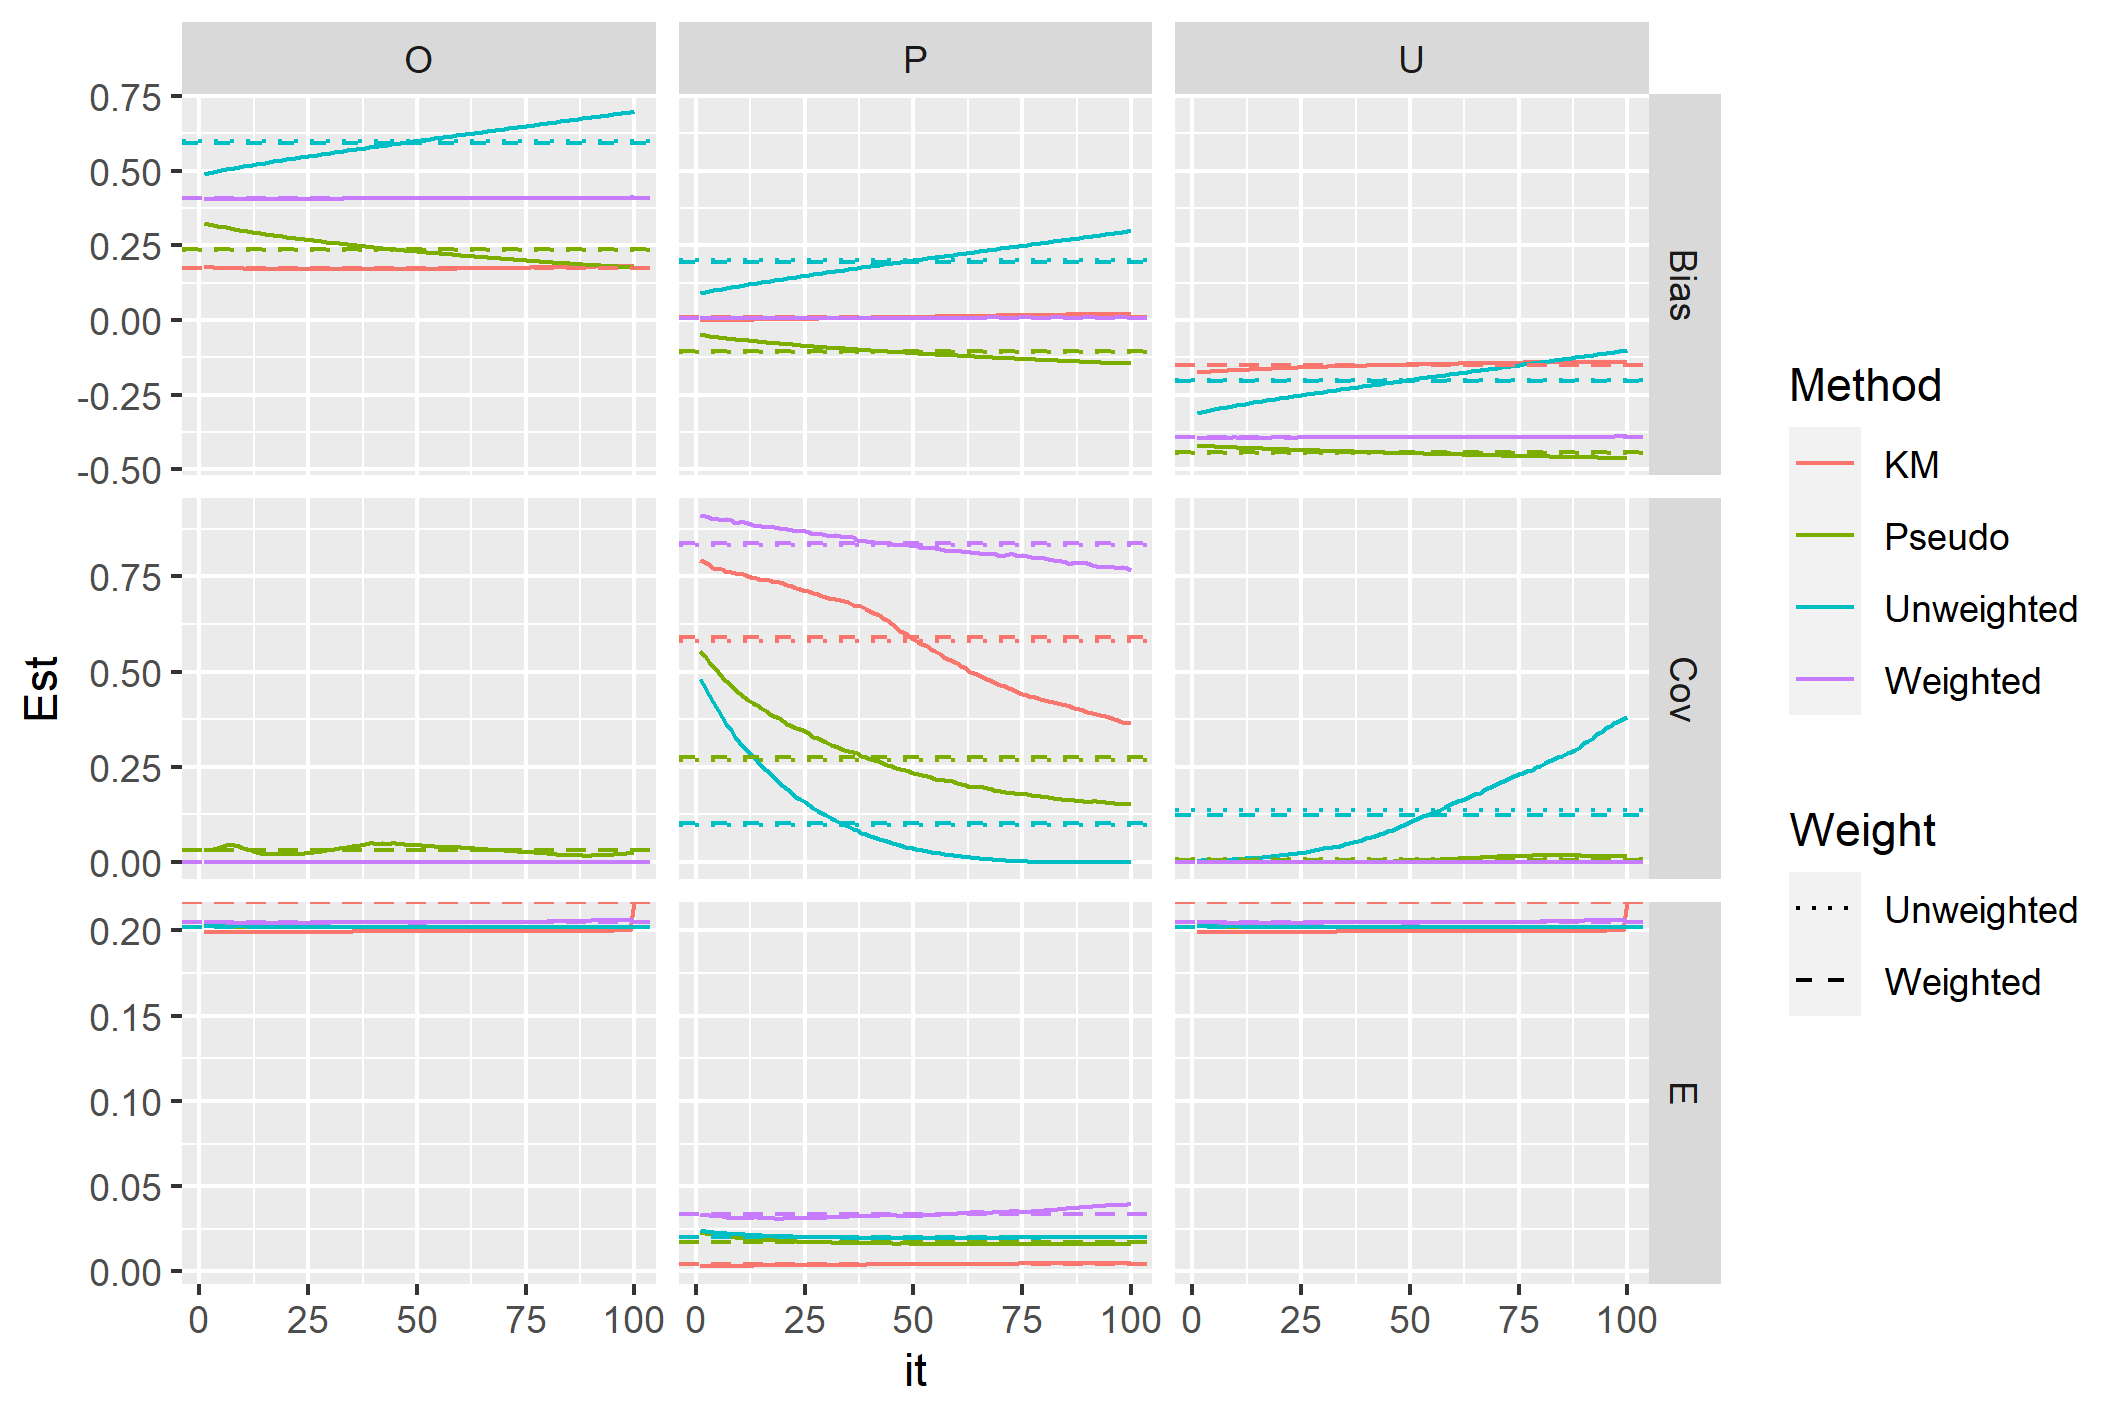
\includegraphics[width=29.51in]{figure/IPCW_Logistic/Main_Plot}

The results in \ref{fig:MainPlot} show the results averaged across all \(\beta\), \(\gamma\) and \(eta\) parameters. In both the Over- and Under-Prediction Models the Bias is closest to zero for the KM Method, with the Weighted remaining constant over time and Pseudo and Unweighted drifting. For Coverage, the none of the models accurately predicted the correct Over- or Under-Prediction value for our estimate, however in the Perfect model, Weighted had the highest Coverage (although still not the expected 95\%). Empirical Standard Error was on average very low for all Methods (with the highest estimate being around 0.15), again KM produced the lowest error.

\hypertarget{discussion-1}{%
\section{Discussion}\label{discussion-1}}

Weighting = Good.

Not Weighting = Bad.

\textbf{limitation}: Maybe the ``True'' \(\theta\) for the under and over predictions were wrong and that would explain the low Coverage.

\hypertarget{appendix-appendices}{%
\appendix}


\hypertarget{chapIPCWlogisticsupp}{%
\section{Supplementary Material}\label{chapIPCWlogisticsupp}}

\hypertarget{calibration-slope}{%
\subsection{Calibration Slope}\label{calibration-slope}}

The main purpose of this paper was to assess the evaluation of calibration-in-the-large at different time points in a time-to-event clinical prediction model. Along with calibration-in-the-large, various methods of calibration can also produce measures of calibration slope. Calibration slope provides an insight into how well the model predicts outcomes across the range of predictions. In an ideal model, the calibration slope would be 1. The Logistic Weighted, Logistic Unweighted and Pseudo-Observation methods described above can provide estimates of the calibration slope. For each of these methods, we first estimate the calibration-in-the-large as above, using a predictor as an offset, then we use this estimate as an offset to predict the calibration slope (without an intercept term).

\hypertarget{results-2}{%
\subsubsection{Results}\label{results-2}}

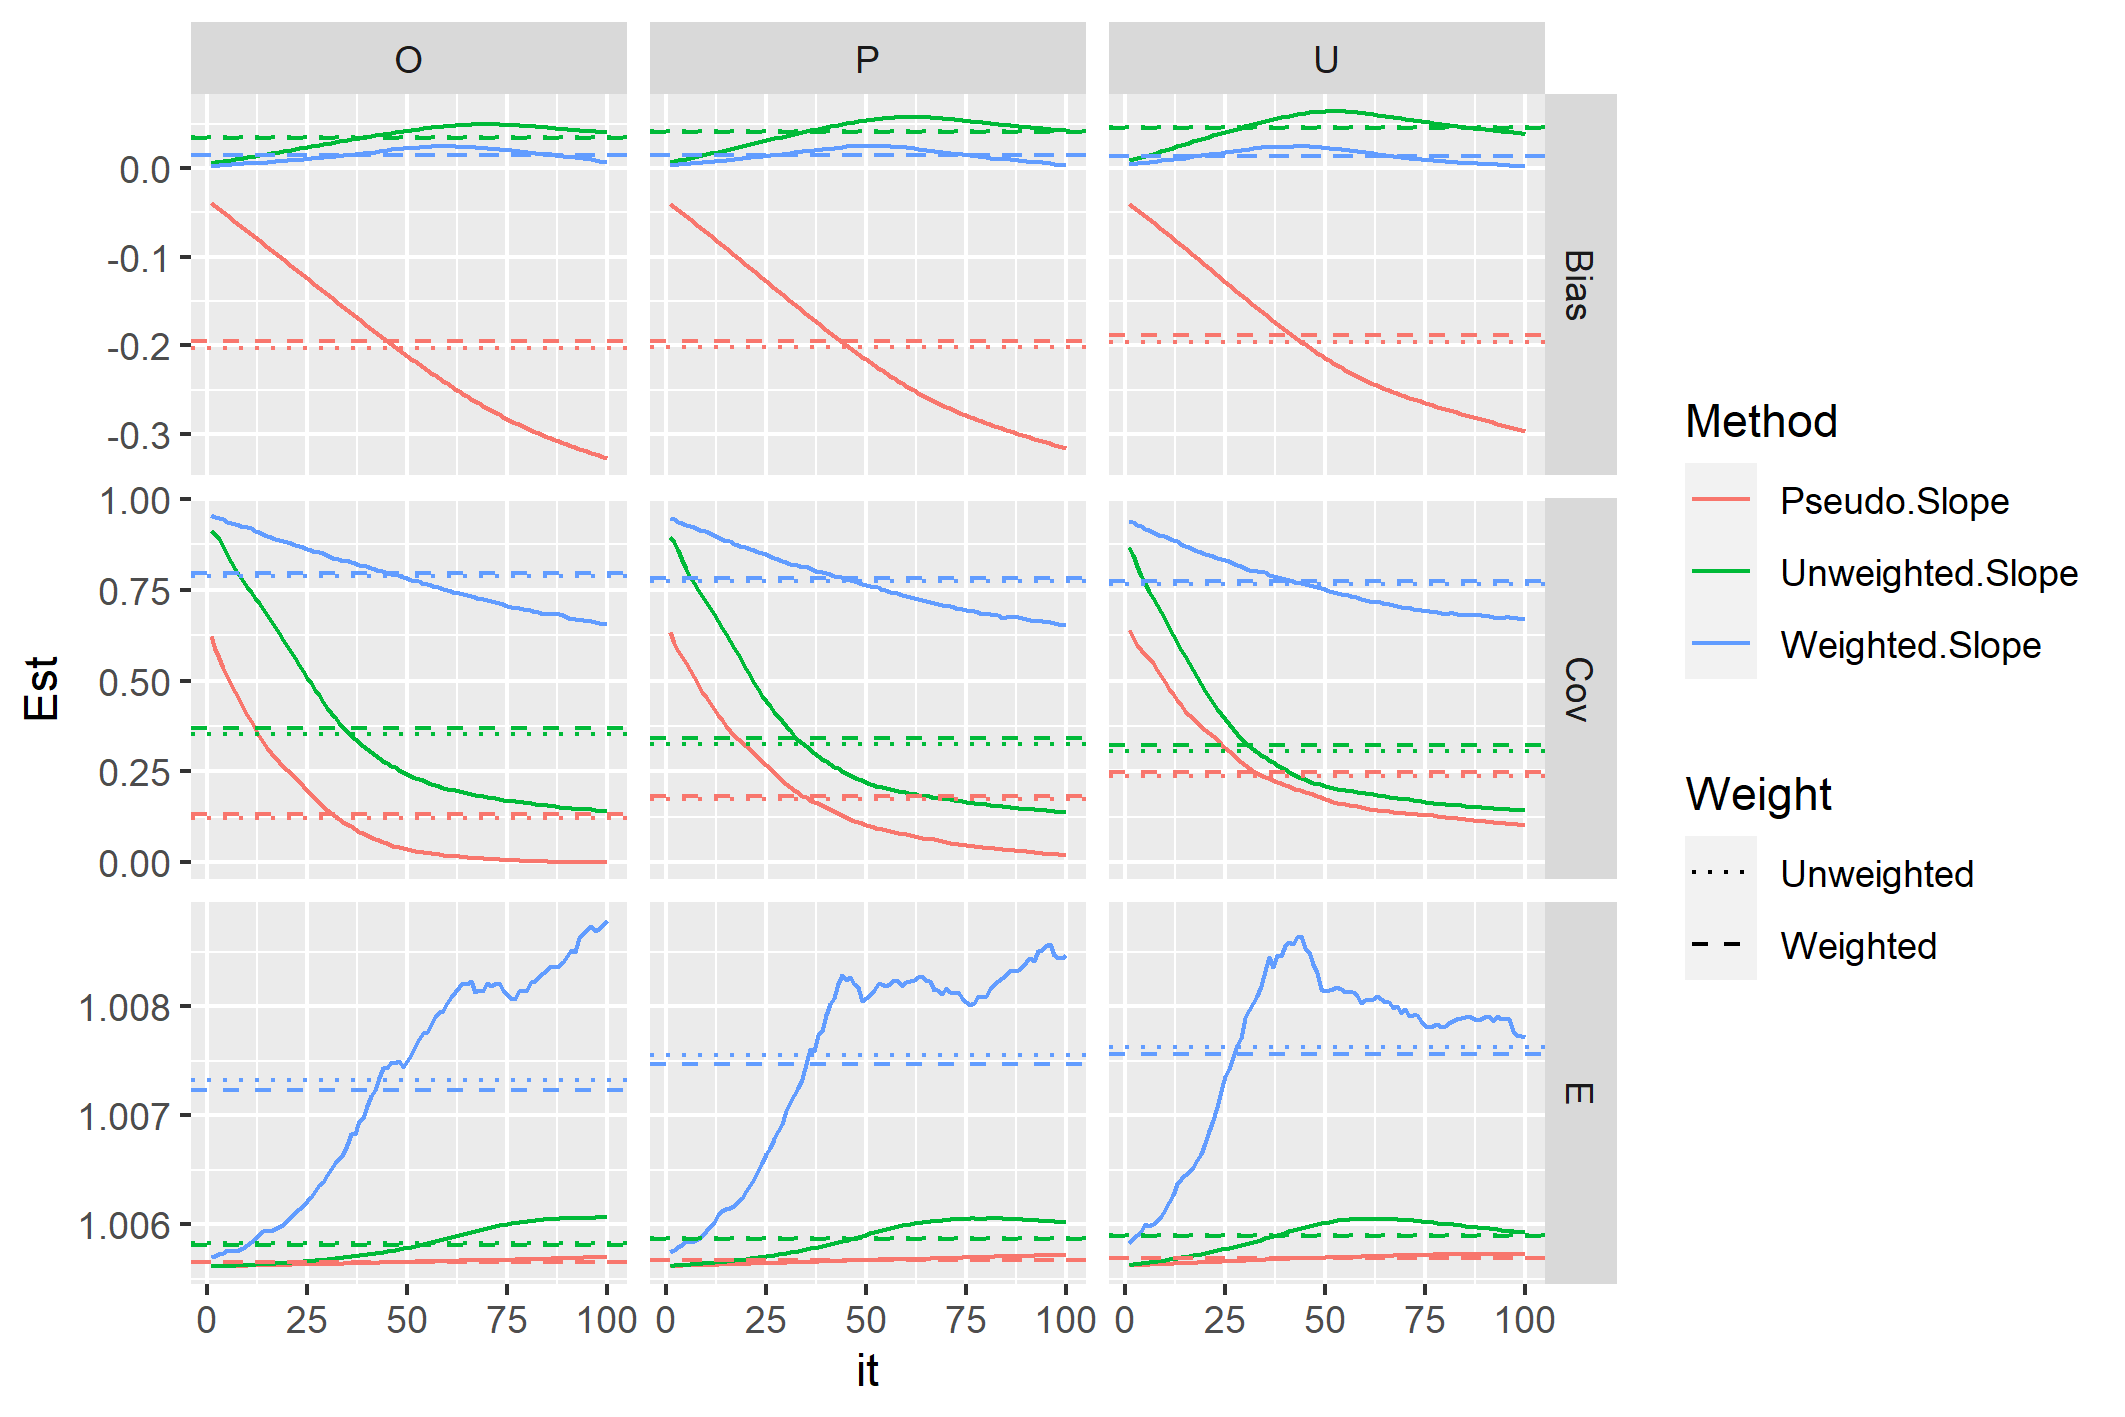
\includegraphics[width=29.51in]{figure/IPCW_Logistic/Slope_Plot}

Results currently show bias/coverage/EmpsE away from 0, rather than 1. Needs fixing. Oops.

\hypertarget{discussion-2}{%
\subsubsection{Discussion}\label{discussion-2}}

Brief discussion, much briefer than the main points.

\hypertarget{references}{%
\section*{References}\label{references}}
\addcontentsline{toc}{section}{References}

\hypertarget{refs}{}
\begin{cslreferences}
\leavevmode\hypertarget{ref-steyerberg_clinical_2008}{}%
{[}1{]} E. W. Steyerberg, \emph{Clinical Prediction Models: A Practical Approach to Development, Validation, and Updating}. Springer Science \& Business Media, 2008.

\leavevmode\hypertarget{ref-calster_calibration_2016-1}{}%
{[}2{]} B. V. Calster, D. Nieboer, Y. Vergouwe, B. D. Cock, M. J. Pencina, and E. W. Steyerberg, ``A calibration hierarchy for risk models was defined: From utopia to empirical data,'' \emph{Journal of Clinical Epidemiology}, vol. 74, pp. 167--176, Jun. 2016, doi: \href{https://doi.org/10.1016/j.jclinepi.2015.12.005}{10.1016/j.jclinepi.2015.12.005}.

\leavevmode\hypertarget{ref-royston_external_2013}{}%
{[}3{]} P. Royston and D. G. Altman, ``External validation of a Cox prognostic model: Principles and methods,'' \emph{BMC Medical Research Methodology}, vol. 13, no. 1, p. 33, Mar. 2013, doi: \href{https://doi.org/10.1186/1471-2288-13-33}{10.1186/1471-2288-13-33}.

\leavevmode\hypertarget{ref-crowson_assessing_2016}{}%
{[}4{]} C. S. Crowson, E. J. Atkinson, and T. M. Therneau, ``Assessing Calibration of Prognostic Risk Scores,'' \emph{Statistical methods in medical research}, vol. 25, no. 4, pp. 1692--1706, Aug. 2016, doi: \href{https://doi.org/10.1177/0962280213497434}{10.1177/0962280213497434}.

\leavevmode\hypertarget{ref-houwelingen_validation_2000}{}%
{[}5{]} H. C. van Houwelingen, ``Validation, calibration, revision and combination of prognostic survival models,'' \emph{Statistics in Medicine}, vol. 19, no. 24, pp. 3401--3415, 2000, doi: \href{https://doi.org/10.1002/1097-0258(20001230)19:24\%3C3401::AID-SIM554\%3E3.0.CO;2-2}{10.1002/1097-0258(20001230)19:24\textless3401::AID-SIM554\textgreater3.0.CO;2-2}.

\leavevmode\hypertarget{ref-hippisley-cox_derivation_2007}{}%
{[}6{]} J. Hippisley-Cox, C. Coupland, Y. Vinogradova, J. Robson, M. May, and P. Brindle, ``Derivation and validation of QRISK, a new cardiovascular disease risk score for the United Kingdom: Prospective open cohort study,'' \emph{BMJ (Clinical research ed.)}, vol. 335, no. 7611, p. 136, Jul. 2007, doi: \href{https://doi.org/10.1136/bmj.39261.471806.55}{10.1136/bmj.39261.471806.55}.

\leavevmode\hypertarget{ref-royston_tools_2014}{}%
{[}7{]} P. Royston, ``Tools for Checking Calibration of a Cox Model in External Validation: Approach Based on Individual Event Probabilities:'' \emph{The Stata Journal}, Dec. 2014, doi: \href{https://doi.org/10.1177/1536867X1401400403}{10.1177/1536867X1401400403}.

\leavevmode\hypertarget{ref-perme_checking_2008}{}%
{[}8{]} M. P. Perme and P. K. Andersen, ``Checking hazard regression models using pseudo-observations,'' \emph{Statistics in medicine}, vol. 27, no. 25, pp. 5309--5328, Nov. 2008, doi: \href{https://doi.org/10.1002/sim.3401}{10.1002/sim.3401}.

\leavevmode\hypertarget{ref-royston_tools_2015}{}%
{[}9{]} P. Royston, ``Tools for Checking Calibration of a Cox Model in External Validation: Prediction of Population-Averaged Survival Curves Based on Risk Groups,'' \emph{The Stata Journal}, vol. 15, no. 1, pp. 275--291, Apr. 2015, doi: \href{https://doi.org/10.1177/1536867X1501500116}{10.1177/1536867X1501500116}.

\leavevmode\hypertarget{ref-hippisley-cox_development_2017}{}%
{[}10{]} J. Hippisley-Cox, C. Coupland, and P. Brindle, ``Development and validation of QRISK3 risk prediction algorithms to estimate future risk of cardiovascular disease: Prospective cohort study,'' \emph{BMJ}, vol. 357, May 2017, doi: \href{https://doi.org/10.1136/bmj.j2099}{10.1136/bmj.j2099}.

\leavevmode\hypertarget{ref-gerds_consistent_2006}{}%
{[}11{]} T. A. Gerds and M. Schumacher, ``Consistent Estimation of the Expected Brier Score in General Survival Models with Right-Censored Event Times,'' \emph{Biometrical Journal}, vol. 48, no. 6, pp. 1029--1040, 2006, doi: \href{https://doi.org/10.1002/bimj.200610301}{10.1002/bimj.200610301}.

\leavevmode\hypertarget{ref-spitoni_prediction_2018}{}%
{[}12{]} C. Spitoni, V. Lammens, and H. Putter, ``Prediction errors for state occupation and transition probabilities in multi-state models,'' \emph{Biometrical Journal. Biometrische Zeitschrift}, vol. 60, no. 1, pp. 34--48, Jan. 2018, doi: \href{https://doi.org/10.1002/bimj.201600191}{10.1002/bimj.201600191}.

\leavevmode\hypertarget{ref-han_comparing_2017}{}%
{[}13{]} X. Han, Y. Zhang, and Y. Shao, ``On comparing two correlated C indices with censored survival data,'' \emph{Statistics in medicine}, vol. 36, no. 25, pp. 4041--4049, Nov. 2017, doi: \href{https://doi.org/10.1002/sim.7414}{10.1002/sim.7414}.

\leavevmode\hypertarget{ref-liu_comparing_2016}{}%
{[}14{]} X. Liu, Z. Jin, and J. H. Graziano, ``Comparing paired biomarkers in predicting quantitative health outcome subject to random censoring,'' \emph{Statistical methods in medical research}, vol. 25, no. 1, pp. 447--457, Feb. 2016, doi: \href{https://doi.org/10.1177/0962280212460434}{10.1177/0962280212460434}.

\leavevmode\hypertarget{ref-burton_design_2006}{}%
{[}15{]} A. Burton, D. G. Altman, P. Royston, and R. L. Holder, ``The design of simulation studies in medical statistics,'' \emph{Statistics in Medicine}, vol. 25, no. 24, pp. 4279--4292, Dec. 2006, doi: \href{https://doi.org/10.1002/sim.2673}{10.1002/sim.2673}.

\leavevmode\hypertarget{ref-riley_prognosis_2019}{}%
{[}16{]} R. D. Riley, D. van der Windt, P. Croft, and K. G. M. Moons, \emph{Prognosis Research in Healthcare: Concepts, Methods, and Impact}, First. Oxford University Press, 2019.

\leavevmode\hypertarget{ref-andersen_pseudo-observations_2010}{}%
{[}17{]} P. K. Andersen and M. Pohar Perme, ``Pseudo-observations in survival analysis,'' \emph{Statistical Methods in Medical Research}, vol. 19, no. 1, pp. 71--99, Feb. 2010, doi: \href{https://doi.org/10.1177/0962280209105020}{10.1177/0962280209105020}.

\leavevmode\hypertarget{ref-morris_using_2019}{}%
{[}18{]} T. P. Morris, I. R. White, and M. J. Crowther, ``Using simulation studies to evaluate statistical methods,'' \emph{Statistics in Medicine}, vol. 38, no. 11, pp. 2074--2102, 2019, doi: \href{https://doi.org/10.1002/sim.8086}{10.1002/sim.8086}.

\leavevmode\hypertarget{ref-r_core_team_r_nodate}{}%
{[}19{]} R. C. Team, ``R: A Language and Environment for Statistical Computing.'' R Foundation for Statistical Computing, Vienna, Austria, Vienna,

\leavevmode\hypertarget{ref-wickham_tidy_2017}{}%
{[}20{]} H. Wickham, ``The tidy tools manifesto.'' https://cran.r-project.org/web/packages/tidyverse/vignettes/manifesto.html, Nov-2017.

\leavevmode\hypertarget{ref-therneau_package_2020}{}%
{[}21{]} T. Therneau, ``A package for survival analysis in R,'' p. 89, Mar. 2020.

\leavevmode\hypertarget{ref-perme_pseudo_2017}{}%
{[}22{]} M. P. Perme, M. Gerster, and K. Rodrigues, ``Pseudo: Computes Pseudo-Observations for Modeling.'' Jul-2017.
\end{cslreferences}
\end{document}
